\subsection{Components of network intensity change}
The 2020--2021 decline in facility-weighted network intensity is the residual of sizeable movements in both directions. Positive net contributions sum to \MiddlePositive{} index points and negative contributions to \MiddleNegative, leaving a net change of $-\MiddleIDecline$. The within-city component is \MiddleWithin{} and the changing-weight component is \MiddleComposition; their partial cancellation explains why a small network-wide movement need not reflect small local changes. All terms are normalized to the initial facility-weighted network intensity of the relevant fixed member set, with the component totals and fixed-member comparison reported in Table~\ref{tab:contributions}.

The city decomposition also separates local intensity from network contribution. Xi'an has the largest negative contribution, \MiddleXianNet{} index points. Chengdu's own within-city component is \MiddleChengduWithin, but its increased facility share contributes \MiddleChengduComposition, producing a positive net contribution of \MiddleChengduNet. Across the 55-city window, 36 cities improve their own intensity, yet only \MiddleNetPositive{} contribute positively to facility-weighted network intensity; \MiddleMismatch{} have opposite signs for own intensity and weighted contribution. A city count and a weighted contribution ranking therefore describe different aspects of the same change (Figure~\ref{fig:contributions}).

The 2022--2023 comparison is less balanced: positive contributions total \RecentPositive{} index points and negative contributions total \RecentNegative. The within-city term is \RecentWithin{} and the weight term is \RecentComposition. The largest five negative contributors account for \RecentNegativeTopShare\% of the negative magnitude, compared with \MiddleNegativeTopShare\% in 2020--2021, but the two windows contain different members and different numbers of negative contributors. A fixed-member check is therefore needed before interpreting concentration as a temporal change.

Holding membership at the common 52 cities, and renormalizing facility weights at every endpoint, gives net intensity changes of \CommonEarlyNet{} and \CommonRecentNet{} index points. Negative weighted contributors increase from \CommonEarlyNegativeN{} to \CommonRecentNegativeN{}; this is a count of negative contributions to facility-weighted network intensity, not a count of cities whose own intensity declined. Their top-five share falls from \CommonEarlyTopFive\% to \CommonRecentTopFive\%, normalized HHI falls from \CommonEarlyHHI{} to \CommonRecentHHI, and the largest fifth comprises \CommonEarlyTopTwentyN{} and \CommonRecentTopTwentyN{} cities with shares of \CommonEarlyTopTwenty\% and \CommonRecentTopTwenty\%. On these fixed-member measures, the later window has a broader distribution of negative contributions. Detailed contribution ranks and concentration statistics are available in SI Section~\siref{sec:si-descriptive}. The comparison describes the observed cities and periods and does not extend to a national trend.
\begin{table}[htbp]\centering\small\caption{City contributions to network intensity}\label{tab:contributions}
\begin{tabular}{@{}p{36mm}rrrr@{}}\toprule & \multicolumn{2}{c}{Window-specific members} & \multicolumn{2}{c}{Same 52 cities}\\\cmidrule(lr){2-3}\cmidrule(lr){4-5}
Quantity & 2020--21 (55) & 2022--23 (93) & 2020--21 (52) & 2022--23 (52)\\
\midrule
Within-city (index points) & -6.160 & -21.666 & -6.091 & -21.162\\
Changing weights (index points) & 5.038 & 2.142 & 4.999 & 1.950\\
Net change (index points) & -1.122 & -19.524 & -1.092 & -19.212\\
Positive contributions (index points) & 8.714 & 4.541 & 8.697 & 3.254\\
Negative contributions (index points) & -9.835 & -24.065 & -9.788 & -22.466\\
Negative contributors & 24 & 49 & 22 & 36\\
Top 5 negative share (\%) & 76.24 & 45.24 & 76.92 & 46.46\\
Normalized HHI & 0.145 & 0.048 & 0.145 & 0.044\\
Largest 20\% share (\%) & 76.24 & 76.49 & 76.92 & 68.40\\
Cities in largest 20\% & 5 & 10 & 5 & 8\\
Own/network signs differ & 15 & 15 & 15 & 7\\
\bottomrule\end{tabular}\end{table}

\begin{figure}[htbp]\centering
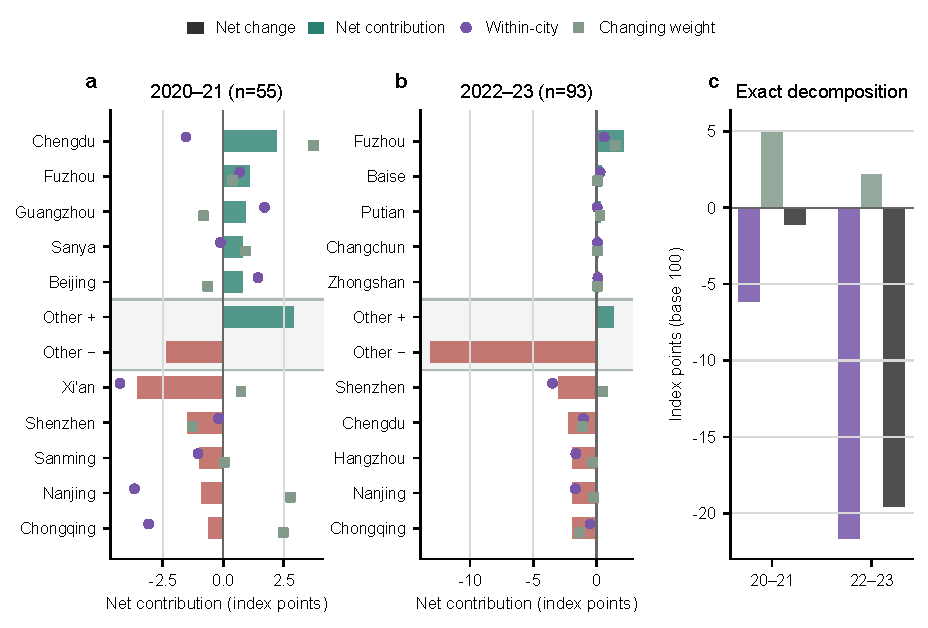
\includegraphics[width=\linewidth,height=.76\textheight,keepaspectratio]{figures/fig5_contributions.pdf}
\caption{City contributions to network intensity}\label{fig:contributions}
\end{figure}

